\documentclass[11pt]{article}
\usepackage[margin=0.75in,landscape]{geometry}
\usepackage{booktabs}
\usepackage{graphicx}
\usepackage[hidelinks]{hyperref}

\title{Supplementary Information: Frequency-Support Requirements for Assessing Direct Ocean-Induced Gravity Signals in Terrestrial Gravimetry}
\author{Hang Diao \and Qikai Zhang \and Yifang Luo \and Wannian Li \and Jiaqing Huang \and Fan Zhang}
\date{}

\begin{document}
\maketitle

\section{Version-controlled analysis protocol}
The configurations are version-controlled analysis protocols rather than an
externally registered clinical-style preregistration. P1-E006 fixes the
1,446-record sensitivity design; P1-E008 fixes the 50, 75, 90 and 95\% energy
fractions; P1-E010 fixes the independent spectral-convention comparison; and
P1-E011 fixes the temporal/spectral convergence audit before its production
execution. Commit hashes, configuration checksums, software environment and
output checksums accompany each experiment. The 20\% Helgoland tolerance was
stored in the P1-E005 protocol before its production output was accepted; it is
an engineering replacement tolerance for differing Earth-response and detiding
implementations, not an observational uncertainty interval.

\section{Process-model parameter registry}
Table~S1 lists every parameter that defines the primary process branches. Ranges
are sensitivity designs and do not define probability distributions.

\begin{table}[ht]
\centering
\caption{Process-model parameters for the P1-E006 direct-radial-gravity ensemble.}
\label{tab:s1-parameters}
\resizebox{\textwidth}{!}{\begin{tabular}{lllll}
\toprule
Process & Parameter & Value/range & Unit & Design interpretation \\
\midrule
Tide & M2 period & $4.471\times10^{4}$ & s & fixed \\
Tide & observation duration & 604800.0--2592000.0 & s & log-midpoint design \\
Tide & disk radius & $1\times10^{5}$ & m & fixed \\
Tide & SSH normalization & 1 & m & geometry diagnostic \\
Eddy & peak SSH anomaly & 0.08 & m & catalogue mean \\
Eddy & horizontal scale & $9\times10^{4}$ & m & fixed \\
Eddy & translation speed & 0.0284185 & m s$^{-1}$ & derived catalogue mean \\
Internal wave & peak density anomaly & 0.4691943732059368--1.1260664956942485 & kg m$^{-3}$ & linear-midpoint sensitivity \\
Internal wave & horizontal scale & 120000.0--129000.0 & m & linear-midpoint sensitivity \\
Internal wave & period & $4.471\times10^{4}$ & s & M2 branch \\
Internal wave & vertical scale / lobe separation & 500.0 / 500.0 & m & exact mass compensation \\
Tsunami & deep-ocean crest amplitude & 1.0--1.8 & m & linear-midpoint sensitivity \\
Tsunami & crest--trough separation & 300000.0--400000.0 & m & linear-midpoint sensitivity \\
Tsunami & source width & $1\times10^{5}$ & m & fixed \\
Tsunami & water depth & 4000 & m & fixed \\
Landslide & slide volume & 2400000000000.0--3000000000000.0 & m$^3$ & linear-midpoint sensitivity \\
Landslide & density contrast & 600 & kg m$^{-3}$ & fixed \\
Landslide & runout & $4.5\times10^{5}$ & m & fixed \\
Landslide & velocity & 30.0--60.0 & m s$^{-1}$ & linear-midpoint sensitivity \\
All idealized families & surface standoff & 10000.0, 30000.0, 100000.0, 300000.0, 1000000.0 & m & fixed design; storm excluded \\
\bottomrule
\end{tabular}
}
\end{table}

\section{Record and spectral registry}
The record duration is $N\Delta t$ under the Fourier convention used by the
software. Before P1-E011, the native frequency spacing is
$\Delta f=(N\Delta t)^{-1}$. Constant detrending removes only the record mean;
no linear detrend is applied to the primary E008 calculation.

\begin{table}[ht]
\centering
\caption{Composition and native temporal resolution of all 1,446 records.}
\label{tab:s2-records}
\resizebox{\textwidth}{!}{\begin{tabular}{lrrrrrr}
\toprule
Process & Records & $N$ range & $\Delta t$ range (s) & Duration range (s) & $\Delta f$ range (Hz) & Nyquist range (Hz) \\
\midrule
internal\_wave & 640 & 65--65 & 1397.32--1397.32 & $9.083\times10^{4}$--$9.083\times10^{4}$ & $1.101\times10^{-5}$--$1.101\times10^{-5}$ & $3.578\times10^{-4}$--$3.578\times10^{-4}$ \\
mesoscale\_eddy & 5 & 65--65 & $3.959\times10^{5}$--$3.959\times10^{5}$ & $2.573\times10^{7}$--$2.573\times10^{7}$ & $3.886\times10^{-8}$--$3.886\times10^{-8}$ & $1.263\times10^{-6}$--$1.263\times10^{-6}$ \\
storm\_surge & 1 & 720--720 & 3600--3600 & $2.592\times10^{6}$--$2.592\times10^{6}$ & $3.858\times10^{-7}$--$3.858\times10^{-7}$ & $1.389\times10^{-4}$--$1.389\times10^{-4}$ \\
submarine\_landslide & 160 & 65--65 & 236.22--461.538 & $1.535\times10^{4}$--$3\times10^{4}$ & $3.333\times10^{-5}$--$6.513\times10^{-5}$ & $1.083\times10^{-3}$--$2.117\times10^{-3}$ \\
tide & 160 & 222--907 & 2794.64--2794.64 & $6.204\times10^{5}$--$2.535\times10^{6}$ & $3.945\times10^{-7}$--$1.612\times10^{-6}$ & $1.789\times10^{-4}$--$1.789\times10^{-4}$ \\
tsunami & 480 & 85--96 & 42.0754--42.0754 & 3576.41--4039.24 & $2.476\times10^{-4}$--$2.796\times10^{-4}$ & 0.0118834--0.0118834 \\
\bottomrule
\end{tabular}
}
\end{table}

\begin{table}[ht]
\centering
\caption{Native-grid lower-frequency requirements. These values are retained
as the P1-E008 result and are subject to the P1-E011 convergence audit.}
\label{tab:s3-frequency}
\resizebox{\textwidth}{!}{\begin{tabular}{lrrrrrr}
\toprule
Process & $f_{50}$ median & $f_{75}$ median & $f_{90}$ min & $f_{90}$ median & $f_{90}$ max & $f_{95}$ median \\
\midrule
internal\_wave & $2.202\times10^{-5}$ & $1.101\times10^{-5}$ & $1.101\times10^{-5}$ & $1.101\times10^{-5}$ & $1.101\times10^{-5}$ & $1.101\times10^{-5}$ \\
mesoscale\_eddy & $3.886\times10^{-8}$ & $3.886\times10^{-8}$ & $3.886\times10^{-8}$ & $3.886\times10^{-8}$ & $3.886\times10^{-8}$ & $3.886\times10^{-8}$ \\
storm\_surge & $4.244\times10^{-6}$ & $1.929\times10^{-6}$ & $7.716\times10^{-7}$ & $7.716\times10^{-7}$ & $7.716\times10^{-7}$ & $3.858\times10^{-7}$ \\
submarine\_landslide & $4.923\times10^{-5}$ & $4.923\times10^{-5}$ & $3.333\times10^{-5}$ & $4.923\times10^{-5}$ & $6.513\times10^{-5}$ & $4.923\times10^{-5}$ \\
tide & $2.207\times10^{-5}$ & $2.152\times10^{-5}$ & $2.005\times10^{-5}$ & $2.147\times10^{-5}$ & $2.204\times10^{-5}$ & $2.136\times10^{-5}$ \\
tsunami & $2.626\times10^{-4}$ & $2.626\times10^{-4}$ & $2.476\times10^{-4}$ & $2.626\times10^{-4}$ & $2.796\times10^{-4}$ & $2.626\times10^{-4}$ \\
\bottomrule
\end{tabular}
}
\end{table}

\section{Instrument evidence}
The three entries are published noise references over their stated intervals,
not complete site-noise models. Their frequency limits are never extrapolated.

\begin{table}[ht]
\centering
\caption{Instrument-noise evidence and frequency support.}
\label{tab:s4-instruments}
\resizebox{\textwidth}{!}{\begin{tabular}{llllll}
\toprule
Instrument/reference & Observable & Band (Hz) & ASD (SI/\sqrt{Hz}) & Evidence type & DOI \\
\midrule
igrav\_quiet\_j9\_self\_noise\_anchor & vertical\_gravity & $1\times10^{-3}$--0.1 & $1\times10^{-9}$ & Approximate flat anchor converted from the paper-reported PSD level. & \url{https://doi.org/10.1093/gji/ggaa359} \\
aqg\_a01\_field\_short\_term\_anchor & vertical\_gravity & $5\times10^{-4}$--0.01 & $7.5\times10^{-7}$ & Flat short-term white-noise anchor only over the explicitly reported plateau. & \url{https://doi.org/10.1038/s41598-018-30608-1} \\
fg5\_228\_short\_term\_anchor & vertical\_gravity & $5\times10^{-4}$--0.01 & $4.5\times10^{-7}$ & Flat short-term white-noise anchor only over the explicitly reported plateau. & \url{https://doi.org/10.1038/s41598-018-30608-1} \\
\bottomrule
\end{tabular}
}
\end{table}

\section{Process constructions and conservation}
The eddy is a Gaussian sea-surface-height anomaly translated parallel to the
idealized coast. The internal-wave branch consists of equal and opposite
three-dimensional Gaussian density lobes, so its discretized net anomalous mass
is zero. Each tsunami record is an equal-mass Gaussian crest--trough pair whose
signed surface mass closes to the stated numerical tolerance. The Storegga
branch removes a solid mass at the source and adds the same mass at the
destination; its transition fraction is a half-cosine ramp. These constructions
are representative forward-model sensitivities, not population models.

\section{Supplementary figures}
\begin{figure}[ht]
\centering
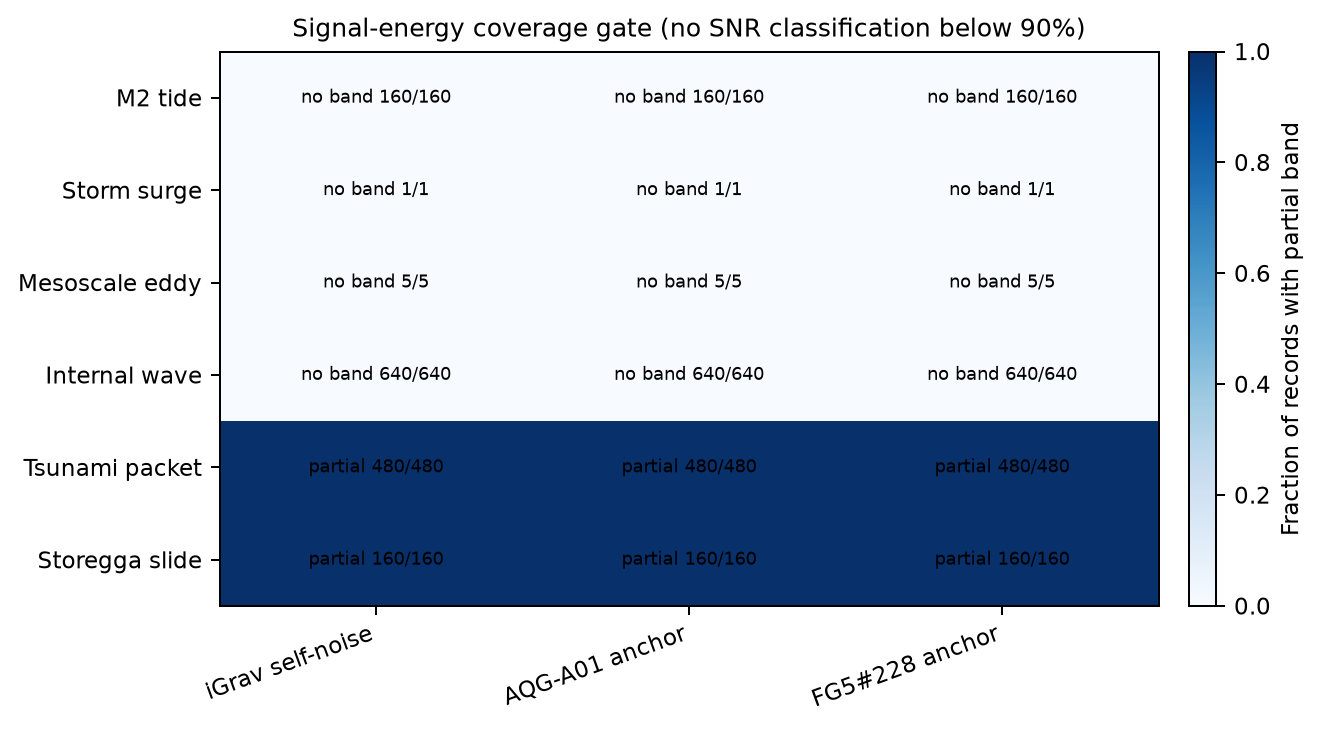
\includegraphics[width=0.88\textwidth]{../../reports/figures/paper1/p1_process_instrument_matrix.png}
\caption{Process--instrument common-support matrix under the original native-bin
implementation. P1-E011 separately reports source Nyquist limitations, native
grid resolution and boundary-aware dense-grid energy coverage.}
\label{fig:s1}
\end{figure}

\begin{figure}[ht]
\centering
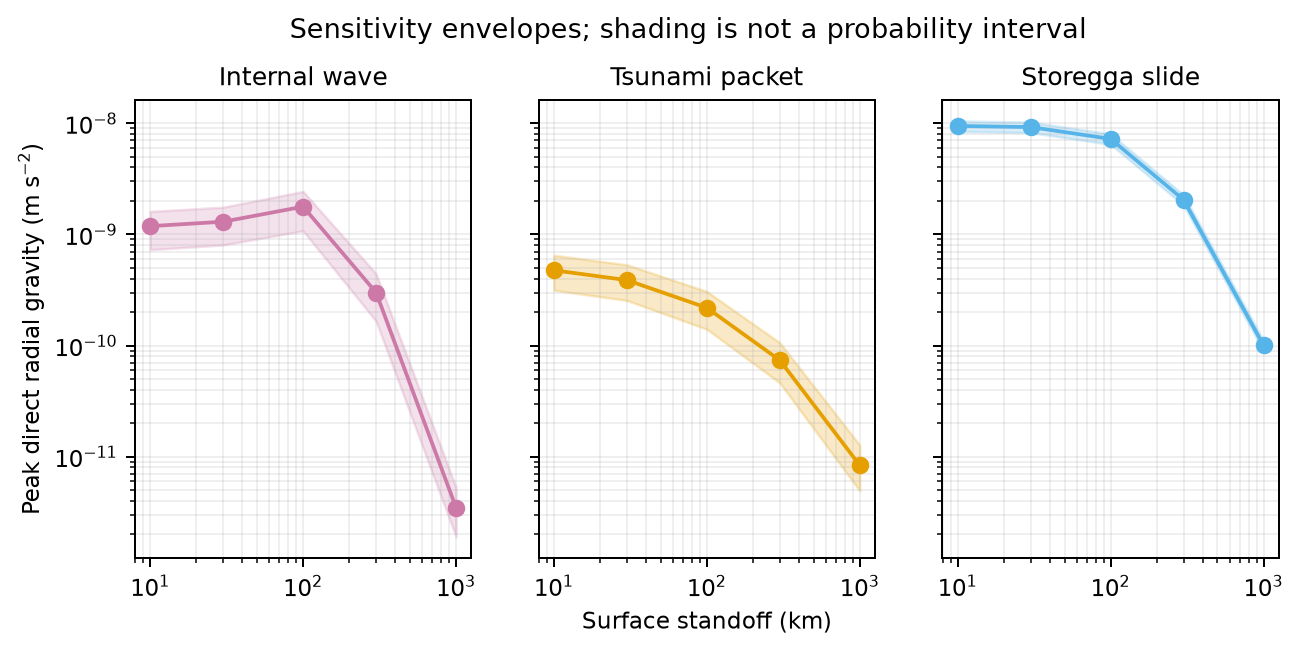
\includegraphics[width=0.88\textwidth]{../../reports/figures/paper1/p1_sensitivity_envelopes.png}
\caption{Version-controlled process sensitivity envelopes. Bands are extrema of
the fixed designs, not confidence or credible intervals.}
\label{fig:s2}
\end{figure}

\end{document}
